\documentclass{article}
\usepackage[utf8]{inputenc}
\usepackage[spanish]{babel}
\usepackage{graphicx}
\usepackage{booktabs}
\usepackage{amsmath, amssymb}
\usepackage{geometry}
\usepackage{hyperref}
\usepackage{caption}
\usepackage{enumitem}
\usepackage{multirow}
\usepackage{float}
\usepackage{fancyhdr} % Paquete para encabezados personalizados
\usepackage{parskip}
\usepackage{tcolorbox}
\usepackage{bold-extra}

\setlength{\parskip}{1em}  % Ajusta la distancia entre párrafos
\setlist[itemize]{noitemsep}
%\setlist[enumerate]{noitemsep}
\captionsetup[figure]{labelfont=bf}
\captionsetup[table]{labelfont=bf}
\geometry{margin=1.3in, headheight=30pt}
\addtolength{\topmargin}{-6.23604pt}

\title{Generalización Proceso de Programación de Actividades en AngloAmerican}
\date{}

\pagestyle{fancy} 
\fancyhf{} 
\lhead{
\includegraphics[width=6cm]{imgs/UC Logo.png}\vspace{1.5mm}} 
\rhead{Emilio Bravo Maturana\\
Magíster en Inteligencia Artificial (c)\vspace{3.5mm}}
\renewcommand{\headrulewidth}{0.4pt} 
\cfoot{\thepage} % Número de página centrado en el pie de página
\renewcommand{\footrulewidth}{0.4pt} % Línea en el pie de página (opcional)

\begin{document}

\begin{titlepage}
\newcommand{\HRule}{\rule{\linewidth}{0.5mm}}
\center
\textsc{\LARGE Pontificia Universidad Católica de Chile}\\[1cm] 
\textsc{\large Magister en Inteligencia Artificial}\\[0.5cm] 
\HRule \\[0.4cm]
\huge \textsc{Desarrollo de un sistema de programación automatizada de tareas para el mantenimiento en la industria minera}\\[0.1cm]
\HRule \\[1cm]
\large\textsc{Emilio Bravo Maturana\\\emph{Profesor Guía: }Rodrigo Sandoval Urrich}\\[1cm]

\includegraphics[scale=0.2]{imgs/UC Logo Grande.png}\\[1cm]
\vfill
{\large\emph{Santiago, Chile. \\ Noviembre 2024 }}\\[2cm]


\end{titlepage}

{\bfseries\scshape Título}\\[.25cm]
Desarrollo de un sistema de programación automatizada de tareas para el mantenimiento en la industria minera.\\


{\bfseries\scshape Autor}\\[.25cm]
Emilio Bravo Maturana\\

{\bfseries\scshape Temática}\\[.25cm]
Programación de Tareas, Algoritmos de Optimización, Resource-Constrained Project Scheduling Problem (RCPSP), Programación por Restricciones y Satisfacción de Restricciones (CP-SAT), Algoritmos Genéticos. 

\newpage

\section*{Resumen}
El mantenimiento eficiente de equipos es crucial para garantizar la continuidad operativa en cualquier industria, pero la programación manual de estas actividades es compleja, intensiva en tiempo y propensa a errores debido a múltiples restricciones y variables. Esto hace que se dependa de personal altamente especializado para la programación de tareas.

Este proyecto, busca optimizar el proceso de programación de tareas de mantenimiento para una empresa del rubro minero, modelándolo como un Problema de Programación de Proyectos con Restricciones de Recursos (RCPSP por sus siglas en inglés). Una correcta generalización del proceso nos permitirá utilizar herramientas de optimización para encontrar una calendarización que cumpla con todas las restricciones del problema, minimizando la función objetivo.

El objetivo es encontrar aquel algoritmo (o set de algoritmos) que permitan encontrar una solución óptima. En un primer acercamiento, utilizaremos algoritmos tipo solver como CP-SAT y algoritmos genéticos. A través de un estudio detallado y pruebas exhaustivas de distintos tipos de algoritmos, se evaluará su desempeño en términos de tiempo de procesamiento, uso de recursos computacionales y calidad de las soluciones obtenidas.

\newpage

\tableofcontents
\newpage
%\maketitle 
%\vspace{-10mm}
%\thispagestyle{fancy} 

\section{Introducción}
\subsection{Contexto}
El mantenimiento de equipos es una actividad fundamental en cualquier industria que busca garantizar la continuidad operativa y la eficiencia en sus procesos productivos. Una planificación adecuada de las actividades de mantenimiento no solo previene fallos inesperados, sino que también optimiza el uso de recursos y minimiza costos asociados a tiempos de inactividad. Sin embargo, la programación eficiente de estas actividades representa un desafío significativo debido a las múltiples restricciones y variables involucradas, como la disponibilidad de personal, recursos materiales, prioridades de tareas y la necesidad de evitar sobreasignaciones y tiempos muertos.

Tradicionalmente, la planificación del mantenimiento ha dependido de equipos humanos que, a pesar de su experiencia y conocimiento, enfrentan limitaciones en términos de tiempo y capacidad para manejar grandes volúmenes de datos y restricciones complejas. Este proceso manual es propenso a errores y puede no garantizar una solución óptima que maximice la eficiencia operativa. En este contexto, surge la necesidad de automatizar este proceso mediante el uso de algoritmos de optimización que puedan abordar de manera efectiva la complejidad inherente de la programación de mantenimiento.

El problema de programación de mantenimiento puede modelarse como un Problema de Programación de Proyectos con Restricciones de Recursos (RCPSP), un enfoque clásico en la investigación operativa para resolver problemas de planificación bajo condiciones de recursos limitados. En este modelo, las tareas de mantenimiento se consideran actividades con duraciones definidas, precedencias entre ellas y recursos compartidos, como personal o maquinaria, cuya disponibilidad es limitada. Las restricciones de precedencia aseguran que ciertas tareas no pueden comenzar hasta que otras hayan finalizado, mientras que las restricciones de recursos garantizan que las capacidades disponibles no sean excedidas en ningún momento. 

El objetivo es encontrar una programación que minimice el tiempo total de ejecución (makespan) o que optimice el uso de recursos, lo que resulta en una planificación más eficiente y acorde con las demandas operativas. Modelar el problema de esta forma permite aplicar algoritmos de optimización avanzados, como los algoritmos genéticos o CP-SAT, para generar soluciones factibles y eficientes.

El presente proyecto tiene como objetivo principal modelar correctamente el problema de programación de mantenimiento y comparar la eficacia y eficiencia de los algoritmos genéticos y los algoritmos CP SAT en su resolución. Para ello, se contará con el apoyo del área de mantenimiento de una empresa del rubro minero, quienes proporcionarán datos reales para realizar las pruebas y ofrecerán retroalimentación a lo largo del desarrollo de la solución. Esta colaboración permitirá ajustar el modelo a las necesidades específicas y desafíos particulares del entorno minero, asegurando que los resultados sean aplicables y relevantes.

\subsection{Consideraciones}
En el contexto de la empresa de del rubro minero, es importante contextualizar la terminología específica utilizada en la programación de tareas. A continuación, se definen algunos términos relevantes para facilitar la comprensión del problema.

\textbf{Orden de Trabajo}: Una orden de trabajo es un conjunto de tareas que se deben realizar para cumplir con un objetivo específico, como el mantenimiento de un equipo o vehículo. Estas órdenes de trabajo se ingresan en el sistema ERP de la empresa y sirven para coordinar y gestionar las actividades de mantenimiento o producción.

\textbf{Número de Operación}: El número de operación hace referencia a las tareas individuales dentro de una orden de trabajo. Estas tareas pueden tener requisitos de precedencia, es decir, algunas deben completarse antes de que otras puedan comenzar. Cada operación cuenta con una fecha de inicio más temprana (earliest date), una fecha requerida de finalización, una duración, una cantidad de trabajadores necesaria y recursos específicos que se requieren para su ejecución.

\textbf{Criticidad}: La criticidad clasifica las tareas según su nivel de prioridad, en una escala del 1 al 3. Las tareas con criticidad 1 son las más urgentes y deben programarse primero, ya que es grave si no se completan dentro de su ventana de tiempo. Las tareas con criticidad 2 y 3 son menos prioritarias y pueden permitirse más flexibilidad en su programación.

\textbf{Cuadrilla}: La cuadrilla representa un grupo de trabajo asignado a una tarea específica dentro de la orden de trabajo. Cada cuadrilla tiene un número determinado de trabajadores y sigue un esquema de turnos específico, trabajando un número fijo de horas por día y un determinado número de días a la semana. La cuadrilla es responsable de ejecutar las operaciones asignadas dentro de su turno.

\textbf{Turno}: El turno define el esquema de trabajo de una cuadrilla. Por ejemplo, un turno 7x7 implica 7 días de trabajo seguidos por 7 días de descanso. Otros esquemas, como el 5x2A, 5x2B o 5x2C, representan 5 días de trabajo con 2 días de descanso, donde las letras A, B y C indican diferentes franjas horarias: A cubre las primeras 8 horas del día, B las siguientes 8, y C las últimas. Estos turnos permiten que las cuadrillas cubran las 24 horas del día de manera continua.


\section{Descripción detallada y levantamiento del problema}
Con el objetivo de automatizar el proceso de programación de tareas en el rubro minero, se llevó a cabo un estudio de los documentos que norman el proceso de programación de tareas en la empresa colaboradora. Este análisis permitió comprender en detalle cómo funciona la programación de tareas en el contexto operativo, y por qué resulta esencial generalizar dicho proceso en un modelo matemático o computacional. Esta generalización es clave, ya que proporciona la base necesaria para desarrollar una herramienta que permita resolver el problema de programación de tareas de manera eficaz y eficiente. El propósito final es implementar una solución automatizada que utilice ya sea un algoritmo de optimización o una red neuronal capaz de entregar resultados satisfactorios.

\subsection{Proceso de Programación}

El proceso de programación en el área de mantenimiento del rubro minero busca garantizar que las tareas se realicen en el momento adecuado, utilizando los recursos de la manera más eficiente posible. Sin embargo, este proceso no opera de manera aislada; previo a la programación, existe un proceso de planificación llevado a cabo por el equipo de planificadores.

\subsubsection{Proceso de Planificación}

El equipo de planificación es responsable de definir, con base en los requerimientos de las máquinas, los tiempos de los procesos industriales, y otros factores relacionados con el negocio minero, las ventanas temporales en las que deben ejecutarse las tareas de mantenimiento. Este proceso considera los objetivos estratégicos de la mina y prioriza el cumplimiento de los requerimientos operativos. Como resultado, se genera una planificación inicial que indica, para cada tarea, la ventana dentro de la cual debe ser realizada. Sin embargo, este proceso no contempla las restricciones de recursos (personal, equipos o herramientas) y asume la disponibilidad de estos en todo momento.

\subsubsection{Proceso de Programación}

El equipo de programación recibe esta planificación inicial como input y realiza un trabajo detallado para adaptarla a las capacidades reales de los recursos disponibles. Su labor principal es balancear los recursos, asegurando que no haya sobreasignaciones y que todas las tareas puedan ser ejecutadas dentro de sus respectivas ventanas. Esto incluye:

\begin{itemize} \item \textbf{Balancear recursos}: Ajustar la programación para que ningún recurso esté sobreexigido y que todas las tareas cuenten con los recursos necesarios para su ejecución. \item \textbf{Asignar fechas y horarios específicos}: Situar con precisión cada tarea en un calendario, definiendo su inicio y fin en función de la disponibilidad de recursos y el cumplimiento de las ventanas definidas por la planificación. \item \textbf{Coordinar accesos}: Garantizar que las cuadrillas, equipos y espacios de trabajo estén disponibles y asignados adecuadamente para cada tarea. \item \textbf{Ajustar y validar la programación}: Consultar a los responsables de ejecución para confirmar la viabilidad del cronograma y obtener su aprobación final. \end{itemize}

El cronograma mínimo resultante detalla las tareas a realizar, los recursos necesarios (personal, equipos y espacios), las condiciones de trabajo, y el impacto de no completar el trabajo en el tiempo establecido. Este proceso también considera tareas en función de su criticidad, priorizando aquellas que tienen mayor impacto en la continuidad operativa.

En eventos complejos, como paradas de planta, la programación se organiza como un proyecto integral que detalla la secuencia de tareas, las dependencias entre ellas, la asignación de recursos especializados, y las actividades de seguimiento y control necesarias para garantizar su éxito. Este trabajo detallado de programación refina y complementa la planificación inicial, adaptándola a las condiciones operativas y logísticas reales.

\subsection{Ciclo Semanal de Programación}

El proceso de programación en el área de mantenimiento se organiza en un ciclo operativo semanal, que se repite de manera sistemática. Este ciclo tiene como objetivo garantizar que el cronograma generado sea factible, actualizado y aprobado por todas las áreas involucradas, de manera que se mantenga alineado con los requerimientos del negocio y la disponibilidad real de recursos.

El ciclo comienza cada miércoles, cuando el equipo de programación toma como base la programación generada la semana anterior. A partir de esta, se revisan las tareas previamente planificadas y programadas, incorporando las nuevas tareas ingresadas durante la semana, así como cualquier cambio en la disponibilidad de recursos. Con esta información, los programadores generan un borrador del cronograma que abarca tres semanas: la semana siguiente y las dos subsiguientes.

Durante este proceso, el borrador es iterado y validado en conjunto con otras áreas involucradas en el proceso de mantenimiento. Este "pinponeo" tiene como objetivo verificar que las tareas estén correctamente distribuidas y que no existan conflictos en la asignación de recursos. Además, permite ajustar el cronograma en función de las prioridades o requerimientos emergentes.

El ciclo culmina cada viernes, cuando se emite el calendario oficial que establece la programación para las tres semanas siguientes. Este calendario sirve como referencia para todas las áreas operativas de la empresa.

\subsubsection{Actualización y Continuidad del Ciclo}

La semana siguiente, el equipo de programación retoma este proceso, partiendo de la base del cronograma generado el viernes anterior. Sin embargo, dado que continuamente ingresan nuevas tareas y los recursos disponibles pueden variar, el equipo revisa y actualiza el cronograma para reflejar estos cambios. Este enfoque iterativo garantiza que la programación se mantenga dinámica y adaptable a las condiciones operativas cambiantes, al tiempo que preserva la continuidad y consistencia en la ejecución de las actividades.

Este ciclo operativo es un componente clave del proceso de programación, ya que asegura que el cronograma se mantenga actualizado y alineado con las necesidades del negocio, mientras se minimizan los conflictos en el uso de recursos. Además, destaca la importancia de la coordinación entre áreas y la validación constante para garantizar un cronograma factible y efectivo.

\subsection{Consideraciones al programar}
El proceso de programación de actividades de mantenimiento implica que el programador tome las órdenes de trabajo pendientes y agende cada una de las tareas considerando su compatibilidad con los horarios y restricciones de otras actividades. Cada tarea viene acompañada de información esencial, asignada en el proceso de planificación, el cual genera los inputs para el proceso de programación. Dentro de esta información tenemos el earliest date (fecha más temprana en la que puede comenzar) y la fecha requerida (plazo máximo de finalización), junto con la cuadrilla asignada para su ejecución. Además, se especifica la duración de la tarea, el número de trabajadores necesarios para llevarla a cabo y su criticidad, que varía de 1 a 3, donde 1 representa la prioridad más alta y debe ser programada de inmediato.

Las tareas utilizan dos tipos de recursos: cuadrillas y equipos. Las cuadrillas tienen características específicas que deben ser gestionadas adecuadamente. Cada cuadrilla trabaja en esquemas de turnos como 7x7, 4x4 o 5x2, lo que indica cuántos días trabajan en cada ciclo, además de si el turno es de día o noche, o si se utiliza el esquema ABC (con tres turnos cubriendo todo el día). Cada cuadrilla tiene una capacidad determinada, que corresponde al número de trabajadores disponibles, lo que influye en la cantidad de tareas que pueden realizarse simultáneamente. Por ejemplo, si una cuadrilla tiene una capacidad de 10 trabajadores, podrá ejecutar 5 tareas que requieran 2 trabajadores cada una de manera simultánea.

Por otro lado, algunos equipos son específicos de cada cuadrilla, por lo que no implican una restricción en el proceso de programación; pero existen recursos compartidos, como grúas y camiones, cuya disponibilidad debe gestionarse cuidadosamente, ya que no pueden estar en dos ubicaciones al mismo tiempo. Por lo tanto, el programador debe coordinar no solo las cuadrillas y sus horarios, sino también la disponibilidad y el uso eficiente de estos equipos compartidos, garantizando que no se generen conflictos o retrasos debido a la sobreasignación de recursos críticos.

\section{Definiciones teóricas}
En este apartado se presentan las definiciones y conceptos teóricos fundamentales para comprender el enfoque del proyecto. Se abordan el Problema de Programación de Proyectos con Restricciones de Recursos (RCPSP), los algoritmos de Programación por Restricciones y Satisfacción de Restricciones (CP SAT), y los algoritmos genéticos. Estos conceptos son esenciales para entender las metodologías utilizadas en la optimización de la programación de actividades de mantenimiento.

\subsection{Problema de Programación de Proyectos con Restricciones de Recursos (RCPSP)}
El RCPSP (Resource-Constrained Project Scheduling Problem) es un problema clásico en el campo de la investigación operativa y la gestión de proyectos. Consiste en programar un conjunto de actividades interrelacionadas, considerando restricciones tanto de precedencia entre tareas como de disponibilidad limitada de recursos. El objetivo principal es determinar el calendario óptimo que minimice la duración total del proyecto (makespan) o que optimice otro criterio relevante, como costos o utilización de recursos.

El RCPSP es conocido por ser un problema NP-Hard, lo que implica que no existe un algoritmo eficiente que pueda resolver todas las instancias del problema en tiempo polinomial. Esta complejidad se debe al crecimiento exponencial del número de posibles soluciones a medida que aumenta el tamaño del problema, es decir, el número de actividades y recursos involucrados. Por esta razón, los métodos exactos son viables solo para problemas de pequeña escala, mientras que para instancias más grandes se recurre a métodos heurísticos y metaheurísticos que proporcionan soluciones aproximadas en tiempos razonables.

Las principales características del RCPSP incluyen:
\begin{itemize}
  \item \textbf{Restricciones de precedencia}: Algunas actividades no pueden comenzar hasta que otras hayan finalizado
  \item \textbf{Recursos limitados}: Los recursos necesarios para realizar las actividades (como mano de obra, equipos o materiales) tienen una disponibilidad limitada en cada periodo de tiempo.
  \item \textbf{Objetivo de optimización}: Generalmente, se busca minimizar el tiempo total del proyecto, aunque pueden considerarse otros objetivos como minimizar costos o equilibrar la carga de recursos.
\end{itemize}

El RCPSP es altamente aplicable en la programación de actividades de mantenimiento industrial, donde es necesario coordinar múltiples tareas con recursos compartidos y restricciones temporales.

\subsection{Algoritmos de Programación por Restricciones y Satisfacción de Restricciones (CP-SAT)}
Los algoritmos de Programación por Restricciones y Satisfacción de Restricciones (CP-SAT) son técnicas avanzadas de optimización que combinan los enfoques de Programación por Restricciones (CP) y Satisfacibilidad Booleana (SAT) para resolver problemas combinatorios complejos, como el Problema de Programación de Proyectos con Restricciones de Recursos (RCPSP). Estos algoritmos son especialmente efectivos debido a su capacidad para manejar de manera eficiente restricciones lógicas, aritméticas y de recursos.

La Programación por Restricciones es un paradigma en el que se definen variables, dominios y restricciones. Las variables representan los elementos desconocidos del problema, los dominios especifican los posibles valores que pueden tomar, y las restricciones limitan las combinaciones de valores que las variables pueden asumir simultáneamente. El objetivo es encontrar asignaciones de valores a las variables que satisfagan todas las restricciones impuestas. Este enfoque es especialmente útil cuando las restricciones son numerosas y complejas, permitiendo modelar problemas de manera flexible y detallada.

Por otro lado, la Satisfacibilidad Booleana (SAT) aborda el problema de determinar si existe una asignación de valores de verdad a variables booleanas que haga verdadera una fórmula lógica dada. Los solucionadores SAT han experimentado avances significativos en eficiencia, lo que permite resolver instancias de gran tamaño en tiempos razonables. La fortaleza de SAT radica en sus algoritmos de búsqueda y propagación altamente optimizados.

La integración de CP y SAT en los algoritmos CP-SAT aprovecha las ventajas de ambos enfoques: la expresividad de CP para modelar problemas con variables y restricciones complejas, y la eficiencia de SAT en la resolución de problemas lógicos. Los algoritmos CP-SAT modelan el problema utilizando variables y restricciones, pero internamente traducen estas restricciones a fórmulas booleanas que pueden ser resueltas eficientemente por un solucionador SAT. Este enfoque híbrido permite manejar problemas con una combinación de restricciones aritméticas y lógicas de manera más eficiente que utilizando solo CP o SAT.

En el contexto del RCPSP, los algoritmos CP-SAT ofrecen un marco poderoso para modelar y resolver el problema de manera eficiente. Se definen variables de inicio y fin para cada tarea, así como variables de intervalo que combinan inicio, duración y fin, facilitando el manejo de restricciones temporales y de recursos. Las restricciones de precedencia se establecen para asegurar que una tarea no pueda comenzar hasta que sus tareas precedentes hayan finalizado, lo cual se expresa mediante relaciones de desigualdad entre las variables de fin e inicio de las tareas involucradas.

Las restricciones de recursos se manejan mediante la restricción cumulativa, que garantiza que, en cualquier momento, la suma de los recursos consumidos por las tareas en ejecución no exceda la capacidad disponible. Esto es crucial en problemas donde los recursos son limitados y deben ser compartidos entre múltiples tareas. Además, se consideran las ventanas de tiempo para las tareas, imponiendo límites en las variables de inicio y fin según las fechas de inicio más tempranas y las fechas límite, lo que refleja la disponibilidad y los plazos específicos de cada tarea.

La función objetivo en estos problemas suele ser minimizar el makespan, es decir, el tiempo total del proyecto. Los algoritmos CP-SAT permiten integrar esta función objetivo en el modelo, buscando no solo soluciones factibles que satisfagan todas las restricciones, sino también optimizar este criterio para mejorar la eficiencia global del proyecto.

Una de las ventajas clave de los algoritmos CP-SAT es su eficiencia en el manejo de restricciones complejas, permitiendo resolver problemas NP-Hard como el RCPSP en tiempos razonables. Su flexibilidad permite incorporar fácilmente nuevas restricciones o modificar las existentes sin reestructurar todo el modelo, lo que es especialmente útil en entornos dinámicos donde las condiciones pueden cambiar. Además, son capaces de encontrar soluciones de alta calidad, óptimas o cercanas al óptimo, lo cual es esencial en contextos industriales donde la optimización de recursos y tiempos es crítica.

\subsection{Algoritmos Genéticos}
Los algoritmos genéticos son una clase de algoritmos metaheurísticos inspirados en los procesos de evolución natural y genética poblacional. Estos algoritmos emulan mecanismos biológicos como la selección natural, el cruce (crossover) y la mutación para explorar el espacio de soluciones de un problema y encontrar soluciones óptimas o cercanas al óptimo.

En problemas de optimización complejos donde el espacio de soluciones es vasto y los métodos exactos son impracticables debido a su complejidad computacional, los algoritmos genéticos ofrecen una alternativa eficiente. Aunque no garantizan encontrar la solución óptima global, su capacidad para explorar múltiples regiones del espacio de soluciones simultáneamente aumenta las probabilidades de acercarse al óptimo en tiempos razonables.

El funcionamiento de un algoritmo genético se basa en la evolución de una población de individuos, donde cada individuo representa una solución potencial al problema. Se comienza generando una población inicial de individuos, generalmente de forma aleatoria, para cubrir una amplia variedad de soluciones posibles. Cada individuo está codificado de una manera que refleja una solución al problema; esta codificación se conoce como cromosoma o genotipo.

Cada individuo es evaluado mediante una función de aptitud (fitness function) que mide qué tan buena es la solución en relación con el objetivo del problema. Esta función es crucial, ya que guía el proceso evolutivo al indicar cuáles individuos son más aptos y, por lo tanto, tienen mayores probabilidades de transmitir sus características a la siguiente generación.

Para generar nuevas soluciones, se aplican operadores genéticos que simulan procesos biológicos:
\begin{itemize}
  \item Selección: Se eligen individuos de la población actual para reproducirse, generalmente dando preferencia a aquellos con mayor aptitud. Métodos comunes incluyen la selección por torneo o por ruleta.
  \item Cruzamiento (Crossover): Se combinan pares de individuos seleccionados para crear descendientes que heredan características de ambos padres. El cruce permite explorar nuevas combinaciones de soluciones y es esencial para recombinar información genética de manera efectiva.
  \item Mutación: Se introducen pequeñas alteraciones aleatorias en los descendientes para mantener la diversidad genética en la población y evitar la convergencia prematura hacia óptimos locales. La mutación ayuda a explorar áreas del espacio de soluciones que podrían no ser alcanzadas solo mediante el cruzamiento.
  
\end{itemize}

La nueva generación de individuos reemplaza parcial o totalmente a la población anterior, dependiendo de la estrategia de reemplazo utilizada. Este proceso se repite durante varias generaciones hasta que se cumple un criterio de parada, como alcanzar un número máximo de generaciones o lograr una aptitud satisfactoria.

El Problema de Programación de Proyectos con Restricciones de Recursos (RCPSP) es un problema complejo de optimización combinatoria, reconocido por ser NP-Hard. Aplicar algoritmos genéticos al RCPSP implica adaptar los componentes del algoritmo para manejar las restricciones específicas del problema, como las precedencias entre tareas, las capacidades limitadas de los recursos y las ventanas de tiempo.
Una de las primeras decisiones al aplicar algoritmos genéticos al RCPSP es cómo representar cada solución (individuo). Una representación común es utilizar una permutación de los IDs de las tareas, que indica el orden en que las tareas serán programadas. Esta permutación debe respetar las restricciones de precedencia; es decir, si una tarea B depende de la finalización de una tarea A, A debe aparecer antes que B en la permutación.


\section{Aplicación de los conceptos teóricos al problema}

\subsection{Problema de Programación}
Con el objetivo de automatizar el proceso de programación de tareas, se llevó a cabo una revisión de los documentos de procedimientos utilizados en la empresa. Este análisis permitió comprender en detalle cómo funciona la programación de tareas en el contexto operativo, y por qué resulta esencial generalizar dicho proceso en un modelo matemático o computacional. Esta generalización es clave, ya que proporciona la base necesaria para desarrollar una herramienta que permita resolver el problema de programación de tareas de manera eficaz y eficiente. El propósito final es implementar una solución automatizada que utilice ya sea un algoritmo de optimización o una red neuronal capaz de entregar resultados satisfactorios.

El proceso de programación en el área de mantenimiento de la empresa busca garantizar que las tareas se realicen en el momento adecuado, utilizando los recursos de la manera más eficiente posible. La programación implica definir el inicio, la secuencia de ejecución y la asignación de recursos (equipos, personal, espacio de trabajo) para cada tarea. Estas deben completarse dentro de una ventana temporal que comienza cuando los recursos están disponibles y finaliza antes de que ocurran consecuencias negativas si no se completan. Cuando surgen conflictos en el acceso a equipos o en la disponibilidad de personal, las decisiones se escalan a los responsables clave.

El objetivo principal de la programación es asignar los recursos necesarios para que todas las tareas aprobadas se completen en el momento oportuno, asegurando un uso eficiente de los recursos. Las actividades relacionadas incluyen definir los tiempos de inicio, coordinar el acceso a equipos y lugares de trabajo, verificar la disponibilidad de personal y herramientas, alinear tareas que se puedan realizar simultáneamente, y consultar a los encargados de ejecutar el trabajo para acordar el cronograma. La programación también incluye gestionar cuestiones críticas y obtener la aprobación de todas las partes involucradas.

El cronograma mínimo debe detallar las tareas a realizar, los equipos y espacios necesarios, las condiciones de trabajo, los recursos requeridos, y el impacto de no completar el trabajo a tiempo. En eventos complejos, como paradas de planta, el cronograma debe organizarse como un proyecto, detallando la secuencia de tareas, dependencias, asignación de recursos especializados y actividades de seguimiento y control.

\subsection{Generalización del Problema como RCPSP}

Vamos a modelar el problema de programación de tareas como un problema de optimización con restricciones, específicamente como una versión del \textit{Resource-Constrained Project Scheduling Problem} (RCPSP). El objetivo es asignar tiempos de inicio a las tareas, maximizando la prioridad de las tareas programadas según su impacto, y respetando las restricciones de capacidad de los recursos, las ventanas de tiempo, los intervalos prohibidos y las posibles relaciones de precedencia entre tareas.

A continuación, se presenta una descripción general del modelo de programación de tareas con recursos limitados que servirá como base para la implementación de la solución.

\subsection*{Parámetros del Modelo}

Tenemos los siguientes elementos:

- \textbf{Tareas}: Un conjunto \( T = \{T_0, T_1, \dots, T_n\} \), donde cada tarea \( T_i \) tiene:
  \begin{itemize}
    \item Una duración \( C(T_i) \in \mathbb{N} \).
    \item Un conjunto de recursos requeridos \( D(T_i) \subseteq R \).
    \item Una cantidad de recurso requerido \( q_i \in \mathbb{N} \).
    \item Un impacto \( \text{Impact}_i \in \mathbb{N} \), donde un valor más bajo indica mayor prioridad.
    \item Una ventana de tiempo \( W(T_i) = [\text{early}_i, \text{late}_i] \), que indica el tiempo más temprano y más tardío en el que puede comenzar la tarea.
  \end{itemize}

- \textbf{Recursos}: Un conjunto \( R = \{R_0, R_1, \dots, R_m\} \), donde cada recurso \( R_j \) tiene:
  \begin{itemize}
    \item Una capacidad \( P(R_j) \in \mathbb{N} \).
    \item Un tipo \( \text{Tipo}(R_j) \in \{0, 1\} \).
    \item Un conjunto de intervalos prohibidos \( I(R_j) = \{[a_1, b_1), [a_2, b_2), \dots\} \), durante los cuales el recurso no está disponible.
  \end{itemize}

- \textbf{Grupos de tareas}: Un conjunto \( G = \{G_0, G_1, \dots\} \), donde cada grupo \( G_k \subseteq T \) tiene restricciones de precedencia entre las tareas que lo componen.

\vspace{0.5cm}

\begin{tcolorbox}[colback=gray!5!white, colframe=gray!75!black, title={Parámetros del modelo}]
    \begin{itemize}
        \item \( T = \{T_0, T_1, \dots, T_n\} \): conjunto de \textbf{tareas}.
        \item \( R = \{R_0, R_1, \dots, R_m\} \): conjunto de \textbf{recursos}.
        \item \( C(T_i) \in \mathbb{N} \): \textbf{duración} de la tarea \( T_i \).
        \item \( D(T_i) \subseteq R \): \textbf{recursos requeridos} por la tarea \( T_i \).
        \item \( q_i \in \mathbb{N} \): \textbf{cantidad} de recurso que requiere la tarea \( T_i \).
        \item \( \text{Impact}_i \in \mathbb{N} \): \textbf{impacto} de la tarea \( T_i \) (prioridad inversa).
        \item \( W(T_i) = [\text{early}_i, \text{late}_i] \): \textbf{ventana de tiempo} para la tarea \( T_i \).
        \item \( P(R_j) \in \mathbb{N} \): \textbf{capacidad} del recurso \( R_j \).
        \item \( \text{Tipo}(R_j) \in \{0, 1\} \): \textbf{tipo} del recurso \( R_j \).
        \item \( I(R_j) = \{[a_k, b_k)\} \): \textbf{intervalos prohibidos} del recurso \( R_j \).
        \item \( G = \{G_0, G_1, \dots\} \): conjunto de \textbf{grupos de tareas} con restricciones de precedencia.
    \end{itemize}
\end{tcolorbox}

\vspace{0.5cm}

\subsection*{Variables de decisión}

Para modelar el problema, introducimos las siguientes variables de decisión:

\begin{itemize}
    \item \( x_i \in \{0, 1\} \): Indica si la tarea \( T_i \) es \textbf{programada} (\( x_i = 1 \)) o no (\( x_i = 0 \)).
    \item \( S_i \in \mathbb{N} \): Tiempo de \textbf{inicio} de la tarea \( T_i \), sujeto a \( \text{early}_i \leq S_i \leq \text{late}_i - C(T_i) \) si \( x_i = 1 \).
    \item \( E_i = S_i + C(T_i) \): Tiempo de \textbf{finalización} de la tarea \( T_i \).
    \item \( \text{Intervalo}(T_i) = [S_i, E_i) \): Intervalo de ejecución de la tarea \( T_i \).
    \item \( y_k \in \{0, 1\} \): Indica si el \textbf{grupo de tareas} \( G_k \) es programado (\( y_k = 1 \)) o no (\( y_k = 0 \)).
\end{itemize}

\vspace{0.5cm}

\begin{tcolorbox}[colback=gray!5!white, colframe=gray!75!black, title={Variables de decisión}]
    \begin{itemize}
        \item \( x_i \in \{0, 1\} \): Variable binaria que indica si la tarea \( T_i \) es \textbf{programada}.
        \item \( S_i \in \mathbb{N} \): Tiempo de \textbf{inicio} de la tarea \( T_i \).
        \item \( E_i = S_i + C(T_i) \): Tiempo de \textbf{finalización} de la tarea \( T_i \).
        \item \( \text{Intervalo}(T_i) = [S_i, E_i) \): Intervalo de ejecución de la tarea \( T_i \).
        \item \( y_k \in \{0, 1\} \): Variable binaria que indica si el grupo \( G_k \) es \textbf{programado}.
    \end{itemize}
\end{tcolorbox}

\vspace{0.5cm}

\subsection*{Restricciones}

El modelo considera las siguientes restricciones:

\textbf{1. Ventanas de tiempo}:

Cada tarea debe comenzar y finalizar dentro de su ventana de tiempo permitida si es programada:

\[
x_i = 1 \implies \text{early}_i \leq S_i \leq \text{late}_i - C(T_i)
\]

\textbf{2. Restricciones de capacidad de los recursos}:

Para cada recurso \( R_j \), la suma de las demandas de las tareas que requieren el recurso en cualquier momento no debe exceder su capacidad:

\[
\sum_{\substack{T_i \in T \\ R_j \in D(T_i)}} q_i \cdot \delta_{ij}(t) \leq P(R_j), \quad \forall t \in \text{Horizonte}
\]

Donde \( \delta_{ij}(t) = 1 \) si \( t \in [S_i, E_i) \) y \( x_i = 1 \); en caso contrario, \( \delta_{ij}(t) = 0 \).

El tipo de recurso afecta cómo se calcula la demanda:

\begin{itemize}
    \item Si \( \text{Tipo}(R_j) = 0 \), se utiliza \( q_i \) como demanda.
    \item Si \( \text{Tipo}(R_j) = 1 \), cada tarea consume una unidad de capacidad (\( q_i = 1 \)).
\end{itemize}

\textbf{3. Intervalos prohibidos de los recursos}:

Las tareas no pueden ser programadas durante los intervalos prohibidos de los recursos que requieren:

\[
x_i = 1 \implies \forall R_j \in D(T_i), \forall [a_k, b_k) \in I(R_j): \quad [S_i, E_i) \cap [a_k, b_k) = \emptyset
\]

\textbf{4. Restricciones de precedencia en grupos de tareas}:

Para cada grupo \( G_k \), si el grupo es programado, las tareas deben seguir una secuencia específica:

\[
y_k = 1 \implies \forall T_i, T_{i+1} \in G_k: S_{i+1} \geq E_i
\]

Además, las tareas dentro de un grupo se programan juntas o no se programan:

\[
\forall T_i \in G_k: x_i = y_k
\]

\textbf{5. Consistencia de variables}:

Si una tarea no es programada, sus variables de tiempo no tienen relevancia y pueden ser fijadas a cero para simplificar el modelo:

\[
x_i = 0 \implies S_i = 0, \quad E_i = 0
\]

\vspace{0.5cm}

\subsection*{Objetivo}

El objetivo es minimizar la penalización asociada a no programar tareas de mayor prioridad. Para esto, se define una función de peso para cada tarea basada en su impacto:

\[
w_i = (\text{Impact}_{\text{max}} + 1 - \text{Impact}_i)^3
\]

Donde \( \text{Impact}_{\text{max}} \) es el valor máximo de impacto entre todas las tareas.

La función objetivo es:

\[
\text{Minimizar } Z = \sum_{i=0}^{n} w_i \cdot (1 - x_i)
\]

Este enfoque penaliza fuertemente la no programación de tareas con mayor prioridad (menor impacto), optimizando así la criticidad global del plan de programación.

\vspace{0.5cm}

\subsection*{Resumen del Modelo}

El modelo presentado integra múltiples aspectos del problema de programación de tareas con recursos limitados:

\begin{itemize}
    \item \textbf{Ventanas de tiempo}: Asegura que las tareas se programen dentro de los intervalos permitidos.
    \item \textbf{Capacidad de recursos}: Garantiza que la demanda no exceda la capacidad disponible en ningún momento.
    \item \textbf{Intervalos prohibidos}: Evita la asignación de tareas durante periodos en los que los recursos no están disponibles.
    \item \textbf{Precedencia en grupos}: Mantiene el orden requerido entre tareas relacionadas.
    \item \textbf{Optimización basada en impacto}: Prioriza la programación de tareas más críticas según su impacto.
\end{itemize}

\subsection{Plan de Desarrollo de la Solución}

La solución se desarrolla de manera modular, estructurándose en tres componentes principales: el backend, el frontend y la integración con las plataformas de la empresa. Esta división permite organizar el flujo de trabajo de forma eficiente y facilita la colaboración con el equipo técnico de la empresa, asegurando que la solución se adapte adecuadamente a sus necesidades.

\begin{figure}[htbp]
  \centering
  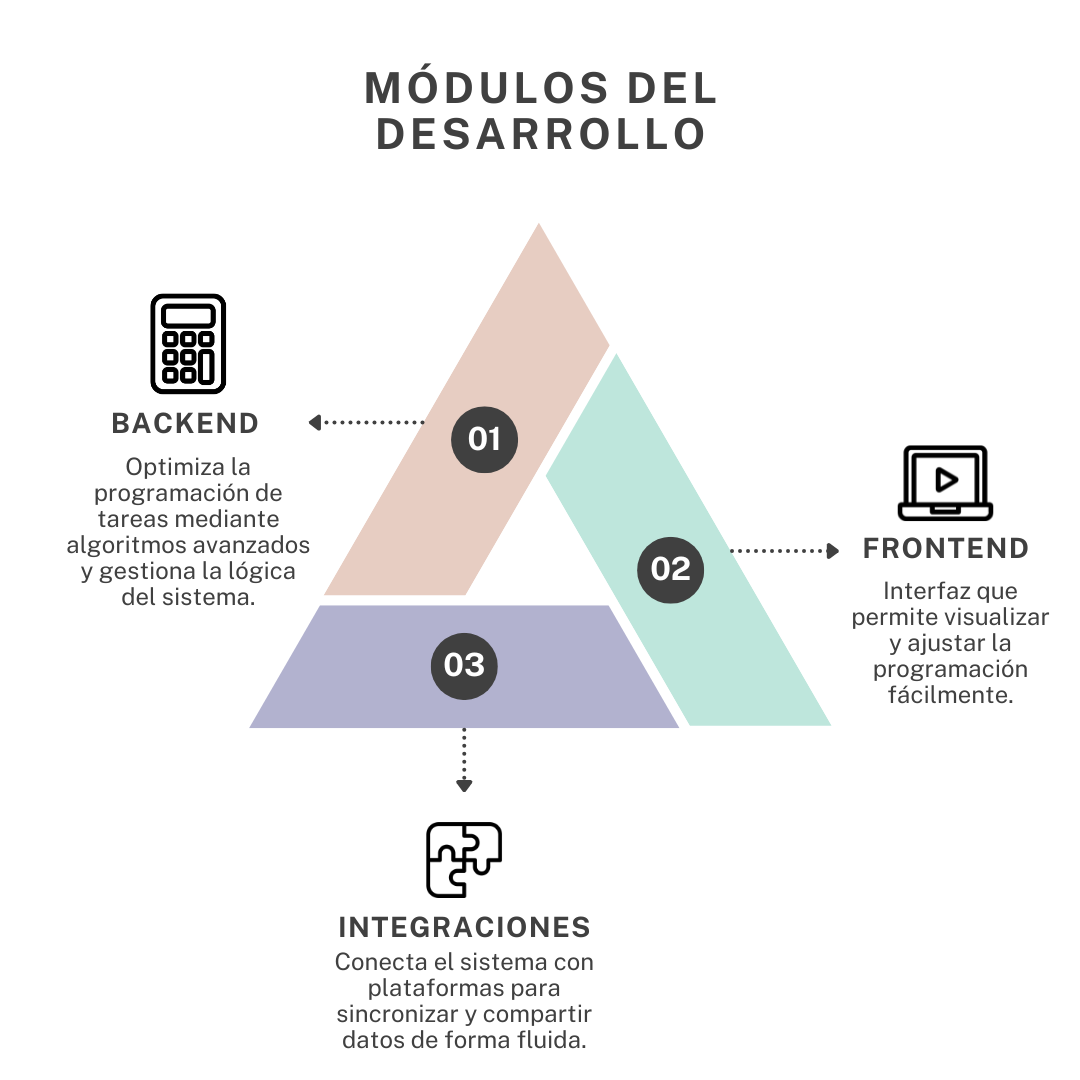
\includegraphics[scale=0.3]{imgs/ModulosDesarrollo.png}
  \caption{Módulos de Desarrollo de Solución}
  \label{fig:modulos-desarrollo}
\end{figure}


\subsubsection{Backend}

El backend representa el núcleo funcional de la solución y ejecuta el algoritmo de programación automatizada de tareas. Este algoritmo se selecciona en función de su capacidad para generar resultados de alta calidad que cumplan con las restricciones y optimicen la programación de tareas según los objetivos planteados. El backend recibe como entrada los datos de las órdenes de trabajo, que incluyen la información específica de cada tarea, tales como duraciones, recursos necesarios, precedencias y ventanas de tiempo.

Alojado en un servicio cloud de la empresa, el backend aprovecha la escalabilidad y el acceso seguro que este entorno proporciona. A partir de los datos ingresados, el backend genera como salida una programación detallada de tareas, especificando para cada una si fue programada y, en caso afirmativo, su hora de inicio. Este módulo se encarga de gestionar la lógica y optimización del proceso de programación, aplicando los algoritmos seleccionados, como CP-SAT, algoritmos genéticos u otros métodos heurísticos y metaheurísticos evaluados.

\subsubsection{Frontend}

El frontend funciona como la interfaz principal para los programadores de la empresa, quienes son los usuarios de esta solución. Su diseño se orienta a la facilidad de uso, permitiendo que los programadores carguen los datos de las órdenes de trabajo de manera sencilla. La carga de datos se puede realizar manualmente o mediante una integración con el sistema ERP de la empresa, de modo que los datos se incorporan automáticamente al sistema.

Una de las funciones clave del frontend es la visualización de la programación de tareas mediante una carta Gantt interactiva, que permite a los usuarios visualizar y, si es necesario, ajustar manualmente la programación generada. Esta funcionalidad ofrece a los programadores la capacidad de evaluar y modificar las tareas programadas antes de aprobar la versión final de la programación. Una vez aprobada, esta información se envía a la plataforma de la empresa, notificando a todos los involucrados sobre la programación establecida.

\subsubsection{Integración con Plataformas de la Empresa}

El tercer módulo se encarga de la integración de la solución con las plataformas de la empresa. Este componente se desarrolla en colaboración estrecha con el equipo de TI de la empresa, asegurando que los formatos de entrada y salida de los datos sean compatibles con los sistemas existentes. La integración también abarca la configuración de conexiones seguras entre el backend y las plataformas corporativas, permitiendo un flujo de información bidireccional. De esta forma, los datos de las órdenes de trabajo y de la programación finalizada se comparten con el ERP y otros sistemas relevantes de la empresa, facilitando la comunicación y coordinación entre los distintos equipos.


\section{Formato de los Datos}

Para desarrollar el sistema de programación automatizada de tareas, trabajaremos con datos extraídos del sistema ERP SAP de la empresa, específicamente en relación con las órdenes de trabajo para el área de mantenimiento. Este sistema proporciona información detallada sobre cada orden de trabajo, incluyendo datos esenciales para la programación de actividades. 

La base de datos con la que se realizará el modelado inicial contiene un total de \textbf{1.098 actividades}, correspondientes a \textbf{239 Órdenes de Trabajo} que deberán programarse dentro de un horizonte de dos semanas. Estás Órdenes de Trabajo corresponden a actividades de mantenimiento preventivo y correctivo en equipos críticos de una de las minas de la empresa para el mes de Julio de 2023.

A continuación, se describen las principales variables presentes en los datos y su función en el modelo de programación:

\begin{itemize}
    \item \textbf{Descripción de la Orden de Trabajo}: Resumen textual de la orden de trabajo, que proporciona contexto general sobre las tareas y objetivos de mantenimiento.

    \item \textbf{Cuadrilla Requerida}: Especifica el grupo de trabajo asignado para la orden de trabajo. Cada cuadrilla tiene sus características específicas, como el tipo de turno y la cantidad de trabajadores disponibles, lo cual se considera en la asignación de actividades.

    \item \textbf{Número de Personas de la Cuadrilla}: Cantidad de trabajadores de la cuadrilla que se requieren para realizar la actividad. Este dato es fundamental para gestionar la capacidad de los recursos humanos y evitar sobreasignaciones.

    \item \textbf{Fecha Requerida}: La fecha límite para completar la actividad. Representa el último momento posible para iniciar y finalizar una actividad sin afectar los planes operativos de la empresa.

    \item \textbf{Fecha de Inicio Extrema}: La primera fecha posible en la que puede comenzar la actividad. Este dato, junto con la fecha requerida, establece la ventana de tiempo permitida para la programación de la actividad.

    \item \textbf{Equipo de Mantenimiento}: Identificación del equipo o maquinaria específica sobre la cual se realizará el mantenimiento. Este dato permite la asignación de recursos específicos y ayuda a gestionar la disponibilidad de los equipos.

    \item \textbf{Impacto (Prioridad)}: Clasificación de la actividad según su criticidad o urgencia, en una escala de 1 a 3, donde 1 representa la máxima prioridad. Este valor orienta el modelo de programación para priorizar las actividades más críticas.

    \item \textbf{Orden de Trabajo}: Número identificador de la orden de trabajo general. Sirve para agrupar varias actividades dentro de un mismo conjunto de trabajo.

    \item \textbf{Número de Actividad}: Identificador único de cada actividad específica dentro de una orden de trabajo. Permite realizar un seguimiento detallado de cada tarea y de su dependencia dentro del contexto general de la orden de trabajo.

    \item \textbf{Descripción de la Actividad}: Descripción específica de cada actividad que detalla su propósito o función, lo que permite a los programadores tener claridad sobre el tipo de tarea a realizar.

    \item \textbf{Duración de la Actividad}: Tiempo estimado necesario para completar la actividad, medido en horas o días. Este dato es esencial para calcular el impacto de cada actividad en el cronograma general y en la asignación de recursos.

\end{itemize}

Esta estructura de datos permitirá modelar cada actividad en el contexto de su orden de trabajo correspondiente, optimizando la asignación de recursos y el cumplimiento de plazos críticos. Los datos se consolidarán y organizarán en una base de datos centralizada, donde cada actividad podrá ser procesada y evaluada en función de las restricciones de recursos y tiempos definidos en el modelo, buscando así maximizar la eficiencia del plan de programación en el horizonte de tres semanas.

\subsection{Entrada de Datos}

El backend recibe como entrada un archivo JSON que contiene la lista completa de tareas a programar. Cada tarea en el JSON incluye los siguientes campos clave:

\begin{itemize}
    \item \textbf{Duración}: Tiempo necesario para completar la tarea, en horas o días.
    \item \textbf{Impacto}: Nivel de prioridad o criticidad de la tarea, que influye en el orden de programación.
    \item \textbf{Cantidad de Personas Necesarias}: Número de trabajadores requeridos para ejecutar la tarea.
    \item \textbf{Cuadrilla Necesaria}: Grupo de trabajo asignado para la tarea, definido según el tipo de turno y la disponibilidad de personal.
    \item \textbf{Herramientas Adicionales Necesarias}: Recursos específicos adicionales, como equipos o maquinaria compartida.
    \item \textbf{Fecha de Inicio Extrema}: La primera fecha en la cual la tarea puede comenzar.
    \item \textbf{Fecha Requerida}: La última fecha en la cual debe completarse la tarea.
\end{itemize}

Además, el backend toma información adicional sobre los recursos, específicamente para cada cuadrilla. Este conjunto de datos incluye:

\begin{itemize}
    \item \textbf{Número de Personas en la Cuadrilla}: Cantidad total de trabajadores disponibles en cada cuadrilla.
    \item \textbf{Esquema de Turno}: Horario laboral de cada cuadrilla, que define el número de días trabajados por semana y la cantidad de horas trabajadas diariamente.
\end{itemize}


\subsection{Salida de Datos}

El resultado de la optimización se genera en un archivo XML, estructurado para ser compatible con herramientas de gestión de proyectos como Microsoft Project. Este archivo XML incluye, para cada tarea:

\begin{itemize}
    \item \textbf{Estado de Programación}: Indica si la tarea fue programada o no.
    \item \textbf{Fecha y Hora de Inicio Programada}: Tiempo de inicio de la tarea en el cronograma.
    \item \textbf{Fecha y Hora de Finalización Programada}: Tiempo de finalización de la tarea.
\end{itemize}

Este archivo XML será utilizado en dos etapas posteriores del flujo de trabajo: se integrará con el frontend para que los programadores puedan revisar y, si es necesario, ajustar manualmente la programación; y se enviará a las plataformas de la empresa mediante el módulo de integración, garantizando que todos los equipos involucrados tengan acceso a la programación finalizada en un formato compatible con los sistemas existentes.


\section{Flujo de Trabajo}

El backend de la solución está diseñado para recibir la información de programación en un formato estructurado, procesarla mediante un algoritmo de optimización y generar como salida una planificación completa que cumpla con las restricciones operativas. Este flujo se divide en varias etapas, que van desde la ingesta de datos hasta la salida de los resultados en un formato compatible con las herramientas de planificación de la empresa.

\subsection{Algoritmo de Programación con Restricciones}


En este caso, la optimización de la programación de actividades en el backend se realiza mediante el uso de \texttt{OR-Tools} y el modelo de programación por restricciones CP-SAT de Google. Este modelo toma como entrada el conjunto de tareas, recursos y restricciones descritas previamente y calcula un cronograma que busca maximizar el cumplimiento de las tareas según sus prioridades y ventanas de tiempo, al mismo tiempo que respeta la disponibilidad de los recursos. A continuación, se describen los elementos técnicos y parámetros clave utilizados en la configuración del modelo.

Para cada tarea, se definen variables que representan su programación, como \texttt{is\_scheduled}, \texttt{task\_starts} y \texttt{task\_ends}. Estas variables almacenan si la tarea es programada, el tiempo de inicio y el tiempo de finalización respectivamente. Adicionalmente, se crean intervalos opcionales \texttt{task\_intervals} que facilitan el manejo de restricciones temporales y la superposición de tareas.

En cuanto a la estructura del código de optimización:

\begin{itemize}
    \item \textbf{Restricciones de Ventanas de Tiempo}: Para cada tarea, el modelo asegura que su tiempo de inicio esté dentro de su ventana temporal permitida. Estas restricciones se implementan mediante variables de intervalo opcional que habilitan o deshabilitan la programación de una tarea según su ventana de tiempo.

    \item \textbf{Restricciones de Intervalos Prohibidos}: Las tareas que requieren recursos específicos deben programarse fuera de los intervalos de tiempo en los que dichos recursos están ocupados o no disponibles. Esto se implementa mediante variables booleanas que indican si una tarea comienza o termina fuera de un intervalo prohibido, las cuales se imponen solo si la tarea es programada.

    \item \textbf{Restricciones Cumulativas para Recursos}: Para cada recurso, el modelo aplica una restricción cumulativa que asegura que el consumo de capacidad por parte de las tareas que lo utilizan no exceda su límite en ningún momento. Se especifica la demanda de cada tarea según el tipo de recurso (con capacidad de 1 unidad o más, dependiendo de la cuadrilla o del equipo adicional), y se controla el consumo de cada recurso con esta restricción.

    \item \textbf{Precedencia en Grupos de Tareas}: En los grupos de tareas (TaskGroup), el modelo aplica restricciones de precedencia entre tareas específicas, asegurando que se respeten los órdenes de ejecución entre ellas si el grupo está programado. Esto se controla mediante la variable booleana \texttt{group\_scheduled}, que activa las restricciones de precedencia dentro de cada grupo solo cuando el grupo completo ha sido asignado al cronograma.
\end{itemize}

La configuración del solucionador CP-SAT incluye dos parámetros clave, \texttt{max\_time\_in\_seconds} y \texttt{relative\_gap\_limit}, que permiten limitar el tiempo de búsqueda y definir un margen de optimalidad aceptable, respectivamente:

\begin{itemize}
    \item \texttt{max\_time\_in\_seconds}: Se establece un límite de tiempo máximo para la búsqueda de soluciones, lo cual ayuda a evitar tiempos de procesamiento prolongados en caso de problemas complejos. En el presente modelo, el límite se ha configurado en 10 segundos, pero puede ajustarse según la demanda de precisión o la disponibilidad de tiempo en un entorno productivo.

    \item \texttt{relative\_gap\_limit}: Este parámetro permite especificar un \textit{gap} relativo de optimalidad que representa el porcentaje aceptable de desviación de la solución encontrada respecto al óptimo teórico. En este caso, se ha fijado en 25\%, lo cual permite una solución razonable en menos tiempo de procesamiento, al aceptar soluciones cercanas al óptimo si el tiempo de ejecución es limitado.
\end{itemize}

La función objetivo está orientada a minimizar la penalización por no programar tareas de alta prioridad. Utilizando una ponderación inversamente proporcional al impacto de cada tarea, el modelo aplica un peso cúbico \((\text{max\_impact} + 1 - \text{impact})^3\) a cada tarea, de modo que las actividades con mayor criticidad se prioricen en el proceso de programación.

El resultado de la optimización se verifica y se genera un archivo XML que contiene el estado de programación de cada tarea, incluyendo las fechas y horas de inicio y finalización si la tarea fue programada. Este archivo, compatible con herramientas de gestión como Microsoft Project, se emplea para visualizar los resultados en el frontend y para integrarse con las plataformas de la empresa mediante el módulo de integración.

\subsection{Algoritmo Genético}
TBA

\subsection{Combinación CP-SAT y Algoritmo Genético}
TBA

\section{Resultados Preliminares}

Para evaluar el desempeño inicial del modelo de programación, se utilizó una base de datos con 1098 actividades, correspondientes a 239 órdenes de trabajo del mes de julio de 2023. Estas actividades fueron procesadas mediante el modelo de optimización CP-SAT de OR-Tools, implementado con los parámetros \texttt{max\_time\_in\_seconds} y \texttt{relative\_gap\_limit} configurados en 10 segundos y 25\%, respectivamente. El objetivo del modelo fue maximizar la cantidad de actividades programadas, respetando las restricciones de recursos y ventanas de tiempo.

\subsection{Resumen de los Resultados}

De las 1098 actividades ingresadas, el modelo logró programar exitosamente 702 actividades (64\% del total), mientras que 396 actividades (36\%) no pudieron ser programadas. La imposibilidad de programar estas últimas actividades probablemente se deba a conflictos en el uso de recursos compartidos, limitaciones de capacidad de las cuadrillas, o solapamientos en las ventanas de tiempo permitidas para cada actividad. Este resultado indica que, bajo las restricciones y los recursos actuales, el modelo encuentra una solución viable para la mayoría de las actividades.

\subsection{Detalles del Proceso de Optimización}

El proceso de optimización fue complejo y se estructuró en diversas etapas clave que permitieron abordar de manera eficiente la cantidad y variedad de restricciones que caracterizan al problema de programación. Para obtener una solución factible, el modelo ejecutó múltiples fases de simplificación y detección de relaciones entre variables y restricciones, lo cual redujo significativamente la cantidad de operaciones necesarias en la etapa de búsqueda. Cada fase del proceso fue diseñada para asegurar que las actividades cumplieran con las restricciones temporales, de capacidad de recursos y de prioridad, mientras se equilibraba el uso de recursos computacionales y se minimizaba el tiempo de resolución.

\begin{itemize}
    \item \textbf{Variables y restricciones}: El modelo trabajó con un total de 407,016 variables, de las cuales 404,820 eran booleanas, y aproximadamente 806,980 restricciones lineales, lo cual refleja la complejidad del problema de programación. Además, se definieron 201,745 restricciones tipo \texttt{kBoolOr} y 1,098 restricciones de intervalo, vinculadas a las actividades programadas.\\

    \item \textbf{Presolución (presolve)}: El solver ejecutó una serie de pasos de presolución, incluyendo detección de relaciones de dominancia y simplificación de restricciones. Esta fase logró reducir el modelo inicial al eliminar 171,592 variables no utilizadas y consolidar restricciones redundantes, lo cual mejoró la eficiencia en la búsqueda de soluciones factibles.\\

    \item \textbf{Iteraciones y subsolvers}: La búsqueda de soluciones involucró varios subsolvers especializados para manejar diferentes aspectos del problema, como \texttt{core}, \texttt{quick\_restart}, y \texttt{no\_lp}. Durante la optimización, se realizaron más de 148,000 ramificaciones y 78 conflictos, lo cual subraya la complejidad de la búsqueda en un espacio tan amplio de soluciones posibles.\\

    \item \textbf{Objetivo y límite de tiempo}: El solver alcanzó un valor objetivo de 1830 al cumplirse el límite de tiempo de 10 segundos y un margen de optimalidad relativo de 25\%. Este límite de tiempo fue útil para obtener soluciones en un tiempo razonable, aunque también dejó un margen de mejora en la programación de actividades adicionales.
\end{itemize}

\section{Conclusiones Preliminares}

El modelo de optimización basado en OR-Tools ha demostrado ser efectivo para programar la mayoría de las actividades bajo restricciones complejas, entregando resultados satisfactorios en un tiempo razonable de 10 segundos. Este desempeño indica que el modelo cumple con los objetivos iniciales de generar un cronograma viable y alineado con las necesidades operativas.

Sin embargo, para hacer la solución más práctica en un entorno de producción en tiempo real, el siguiente desafío es reducir el tiempo de ejecución a un valor cercano a la instantaneidad. Para lograrlo, se incorporarán técnicas de algoritmos genéticos, que permitirán explorar el espacio de soluciones de manera más rápida y adaptable.

Asimismo, será clave el desarrollo de un frontend que permita a los usuarios visualizar, editar y aprobar la programación de forma intuitiva, integrando la solución a la operación diaria de la empresa. Estos pasos adicionales completarán el sistema, optimizándolo tanto en tiempos de respuesta como en facilidad de uso.



\end{document}
